\subsection*{Основные формулы}

\textbf{Спектр водорода}. 
Длины волн спектральных линий водорода описываются формулой Бальмера:
\begin{equation}\label{Balmer}
\dfrac{1}{\lambda_{mn}} = R \left( \dfrac{1}{n^2} - \dfrac{1}{m^2} \right),
\end{equation}
где $R$ -- постоянная Ридберга. 
В работе изучается серия Бальмера, т.е. переходы при $ n = 2 $ и линии $ m = 3, 4, 5$, обозначаемые как $ H_\alpha, H_\beta, H_\gamma$.
    

\textbf{Спектр йода}. 
% Оптические переходы 
% (переходы, связанные с излучением фотонов в видимом диапазоне длин волн, т. е. фотонов с энергией порядка двух электрон-вольт) 
% соответствуют переходам между различными электронными состояниями молекулы. При этом обычно происходят также изменения ее вращательного и колебательного состояний. 
Энергетическое положение линий поглощения описывается выражением (см. рис \ref{fig:33})
\begin{equation}\label{iod}
h\nu_{(0,n_2)} = E_2 - E_1 + h\nu_2 \left( n_2 + \dfrac{1}{2} \right) - \dfrac{h \nu_1}{2}
\end{equation}

\begin{figure}[h]
    \centering
    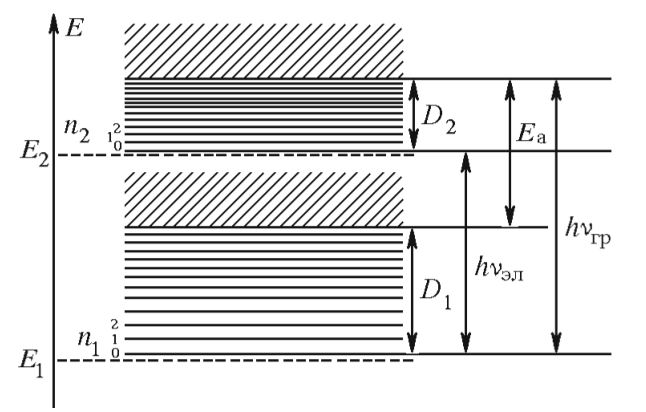
\includegraphics[width=0.45\textwidth]{iod.png}
    \caption{Электронные и электронно-колебательные энергетические уровни двухатомной молекулы}
    \label{fig:33}
\end{figure}
